\documentclass[12pt, titlepage]{article}

\usepackage{booktabs}
\usepackage{tabularx}
\usepackage{hyperref}
\usepackage{graphicx}
\usepackage{float}
\usepackage{mdframed}
\usepackage{framed}
\usepackage{fancybox}
\newcolumntype{L}{>{\centering\arraybackslash}m{3cm}}
\newcolumntype{C}{>{\centering\arraybackslash}m{5cm}}
\newcolumntype{R}{>{\centering\arraybackslash}m{5cm}}

\hypersetup{
    colorlinks,
    citecolor=black,
    filecolor=black,
    linkcolor=red,
    urlcolor=blue
}
\usepackage[round]{natbib}



\title{SE 3XA3: Requirements Document\\MacSidenotes}

\author{Team 4
		\\ Josh Mitchell mitchjp3
		\\ Matthew Shortt shorttmk
}

\date{\today}

%\input{../Comments}

\begin{document}

\maketitle

\pagenumbering{roman}
\tableofcontents
\listoftables
\listoffigures



\begin{table}[bp]
\caption{\bf Revision History}
\begin{tabularx}{\textwidth}{p{3cm}p{2cm}X}
\toprule {\bf Date} & {\bf Version} & {\bf Notes}\\
\midrule
Oct 6th & 1.0 & Completed before implementation\\
%Date 2 & 1.1 & Notes\\
\bottomrule
\end{tabularx}
\end{table}

\newpage

\pagenumbering{arabic}

%\newmdenv[linecolor=black]{reqbox}

This document describes the requirements for ....  The template for the Software
Requirements Specification (SRS) is a subset of the Volere
template~\citep{RobertsonAndRobertson2012}.  If you make further modifications
to the template, you should explicity state what modifications were made.

\section{Project Drivers}

\subsection{The Purpose of the Project}

\subsection{The Stakeholders}

\subsubsection{The Client}

\subsubsection{The Customers}

\subsubsection{Other Stakeholders}

\subsection{Mandated Constraints}

\subsection{Naming Conventions and Terminology}

\subsection{Relevant Facts and Assumptions}

User characteristics should go under assumptions.

\section{Functional Requirements}

\subsection{The Scope of the Work and the Product}

\subsubsection{The Context of the Work}

	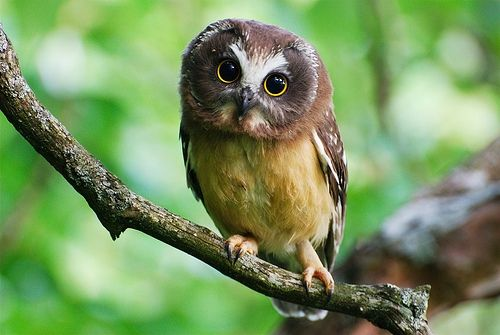
\includegraphics[width=\linewidth]{images/owl.jpg}
	*Note: Replace owl with actual diagram


\subsubsection{Work Partitioning}
\begin{table}[bp]
		\setlength{\extrarowheight}{1ex}
	\caption {\bf Business Event List}
	\begin{tabularx}{\textwidth}{L|C|R}
		{\bf Event Name} & {\bf Input and Output} & {\bf Summary of BUC}\\
		\hline
		1. User clicks extension icon & Button click event (in) \newline Sidebar popup (out) & Extension sidebar pops out.\\
		2. User types in sidebar & Keystrokes (in) \newline Text in sidebar (out) & Note is displayed as it is being entered.\\
		
	\end{tabularx}

\end{table}

\subsubsection{Individual Product Use Cases}

\subsection{Functional Requirements}
\begin{framed}
	
	\begin{center}
		
		\begin{tabular}{ l c r }
			Requirement \#: F.1 & Requirement Type: 9 & Event/Use case \#: \\
		\end{tabular} \\
	\end{center}
	\textbf{Description:} The product should have an attractive html interface. \\
	\\
	\textbf{Rationale:} The product must aesthetically pleasing and easy to use
	to benefit the end-users \\
	\textbf{Originator:} Josh Mitchell \\
	\textbf{Fit Criterion:} Stakeholder satisfaction regarding the appearance  \\
	
	\begin{tabular}{ll}
		\textbf{Customer Satisfaction:} 5 & \textbf{Customer Dissatisfaction:} 5 \\
		\textbf{Priority:} High & \textbf{Conflicts:} None\\
	\end{tabular} \\
	\\
	\textbf{Supporting Materials:} None \\
	\textbf{History:} Created October 5, 2016
	
\end{framed}

\section{Non-functional Requirements}

\subsection{Look and Feel Requirements}


\begin{framed}

	\begin{center}
		
		\begin{tabular}{ l c r }
			Requirement \#: NF.1 & Requirement Type: 10 & Event/Use case \#: \\
		\end{tabular} \\
	\end{center}
	\textbf{Description:} The product should have an attractive html interface. \\
	\\
	\textbf{Rationale:} The product must aesthetically pleasing and easy to use
	to benefit the end-users \\
	\textbf{Originator:} Matthew Shortt \\
	\textbf{Fit Criterion:} Stakeholder satisfaction regarding the appearance  \\

	\begin{tabular}{ll}
		\textbf{Customer Satisfaction:} 5 & \textbf{Customer Dissatisfaction:} 5 \\
		\textbf{Priority:} High & \textbf{Conflicts:} None\\
	\end{tabular} \\
	\\
	\textbf{Supporting Materials:} None \\
	\textbf{History:} Created October 5, 2016

\end{framed}





\subsection{Usability and Humanity Requirements}

\subsection{Performance Requirements}

\subsection{Operational and Environmental Requirements}

\subsection{Maintainability and Support Requirements}

\subsection{Security Requirements}

\subsection{Cultural Requirements}

\subsection{Legal Requirements}

\subsection{Health and Safety Requirements}

This section is not in the original Volere template, but health and safety are
issues that should be considered for every engineering project.

\section{Project Issues}

\subsection{Open Issues}

\subsection{Off-the-Shelf Solutions}

\subsection{New Problems}

\subsection{Tasks}

\subsection{Migration to the New Product}

\subsection{Risks}

\subsection{Costs}

\subsection{User Documentation and Training}

\subsection{Waiting Room}

\subsection{Ideas for Solutions}

\bibliographystyle{plainnat}

\bibliography{SRS}

\newpage

\section{Appendix}

This section has been added to the Volere template.  This is where you can place
additional information.

\subsection{Symbolic Parameters}

The definition of the requirements will likely call for SYMBOLIC\_CONSTANTS.
Their values are defined in this section for easy maintenance.


\end{document}